\documentclass[a4paper,12pt,obeyspaces,spaces,hyphens]{article}

\usepackage{agenda}
\usepackage{colortbl}
\usepackage{xcolor}
\usepackage{calc}

\hypersetup{pdftitle={Buildroot training},
  pdfauthor={Bootlin}}

\renewcommand{\arraystretch}{2.0}

\begin{document}

\thispagestyle{fancy}

\setlength{\arrayrulewidth}{0.8pt}

\begin{center}
\LARGE
Embedded Linux development with Buildroot training\\
\large
3-day session
\end{center}
\vspace{1cm}

\small
\newcolumntype{g}{>{\columncolor{fedarkblue}}m{4cm}}
\newcolumntype{h}{>{\columncolor{felightblue}}X}

\arrayrulecolor{lightgray} {
  \setlist[1]{itemsep=-5pt}
  \begin{tabularx}{\textwidth}{|g|h|}
    {\bf Title} & {\bf Embedded Linux development with Buildroot training} \\
    \hline

    {\bf Overview} &
    Introduction to Buildroot \par
    Managing and building the configuration \par
    Buildroot source and build trees \par
    Toolchains in Buildroot \par
    Managing the Linux kernel configuration \par
    Root filesystem \par
    Download infrastructure \par
    GNU Make 101 \par
    Integrating new packages \par
    Advanced package aspects \par
    Analyzing the build \par
    Advanced topics \par
    Application development with Buildroot \par
    Understanding the Buildroot internals \par
    Buildroot community: support and contribution \par
    What's new in Buildroot? \\
    \hline
    {\bf Materials} &
    Check that the course contents correspond to your needs:
    \newline \url{https://bootlin.com/doc/training/buildroot}. \\
    \hline

    {\bf Duration} & {\bf Three} days - 24 hours (8 hours per day).
    \newline 40\% of lectures, 60\% of practical labs. \\
    \hline

    {\bf Trainer} & {\bf Thomas Petazzoni}. Thomas is a major
    Buildroot developer since 2009, with more than 2700 patches
    integrated and an active participation to the development process.\\
    \hline

    {\bf Language} & Oral lectures: English, French.
    \newline Materials: English.\\
    \hline

    {\bf Audience} & Companies already using or interested in using
    Buildroot to build their embedded Linux systems.\\
    \hline

    {\bf Prerequisites} & {\bf Knowledge of embedded Linux} as covered
    in our embedded Linux course:
    \newline \url{https://bootlin.com/training/embedded-linux/} \vspace{1em}
    \newline {\bf Knowledge and practice of UNIX or GNU/Linux commands}
    \newline People lacking experience on this topic should get
    trained by themselves, for example with our freely available
    on-line slides:
    \newline \url{https://bootlin.com/blog/command-line/} \\
    \hline
  \end{tabularx}

  \begin{tabularx}{\textwidth}{|g|h|}
    {\bf Required equipment} &
    {\bf For on-site sessions only.}
    \newline Everything is supplied by Bootlin in public
    sessions.
    \begin{itemize}
    \item Video projector
    \item PC computers with at least 8 GB of RAM, and Ubuntu Linux
    installed in a {\bf free partition of at least 30 GB. Using Linux
      in a virtual machine is not supported}, because of issues
    connecting to real hardware.
    \item We need Ubuntu Desktop 16.04 (Xubuntu and other
    variants are fine). We don't support other
    distributions, because we can't test all possible package versions.
    \item {\bf Connection to the Internet} (direct or through the
    company proxy).
    \item {\bf PC computers with valuable data must be backed up}
    before being used in our sessions.  Some people have already made
    mistakes during our sessions and damaged work data.
    \end{itemize}\\
    \hline

    {\bf Materials} & Electronic copies of presentations and
    labs.
    \newline Electronic copy of lab files.\\
    \hline

\end{tabularx}}
\normalsize

\feagendatwocolumn
{Hardware}
{
  The hardware platform used for the practical labs of this training
  session is the {\bf BeagleBone Black}, which features:

  \begin{itemize}
  \item An ARM AM335x processor from Texas Instruments (Cortex-A8
    based), 3D acceleration, etc.
  \item 512 MB of RAM
  \item 2 GB of on-board eMMC storage
	\newline(4 GB in Rev C)
  \item USB host and device
  \item HDMI output
  \item 2 x 46 pins headers, to access UARTs, SPI buses, I2C buses
    and more.
  \end{itemize}
}
{}
{
  \begin{center}
    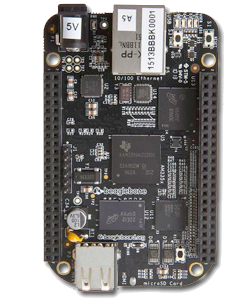
\includegraphics[height=5cm]{../slides/beagleboneblack-board/beagleboneblack.png}
  \end{center}
}

\section{Day 1 - Morning}

\feagendatwocolumn
{Lecture - Embedded Linux and build system introduction}
{
  \begin{itemize}
  \item The general architecture of an embedded Linux system
  \item Build systems vs. binary distributions
  \item Role of a build system
  \item Comparison of existing build systems
  \end{itemize}
}
{Lecture - Introduction to Buildroot}
{
  \begin{itemize}
  \item Key facts about the project
  \item Getting Buildroot
  \item Basic configuration of Buildroot
  \item Doing a first build
  \end{itemize}
}
\\
\feagendatwocolumn
{Lab - Basic Buildroot usage}
{
  \begin{itemize}
  \item Getting and setting up Buildroot
  \item Configuring and building a basic system with Buildroot for the
    BeagleBone Black
  \item Flash and test the generated system on the BeagleBone Black
  \end{itemize}
}
{Lecture - Managing the build and configuration}
{
  \begin{itemize}
  \item Out of tree build
  \item Using and creating {\em defconfigs}
  \item Defconfig fragments
  \item Other building tips
  \end{itemize}
}

\section{Day 1 - Afternoon}


\feagendatwocolumn
{Lecture - Buildroot source and build trees}
{
  \begin{itemize}
  \item Details about the Buildroot source code organization
  \item Details about the Buildroot build tree
  \end{itemize}
}
{Lecture - Toolchains in Buildroot}
{
  \begin{itemize}
  \item The different choices for using toolchains in Buildroot
  \item Overview of the toolchain options
  \item Using existing binary toolchains, such as Sourcery CodeBench
    toolchains, understanding {\em multilib} capabilities and
    integration of toolchains in Buildroot
  \item Generating custom toolchains with {\em Crosstool-NG}, and
    re-use them as external toolchains
  \end{itemize}
}

\feagendatwocolumn
{Lecture - Managing the Linux kernel configuration}
{
  \begin{itemize}
  \item Loading, changing and saving the kernel configuration
  \end{itemize}
}
{Lecture - Root filesystem construction in Buildroot}
{
  \begin{itemize}
  \item Understand how Buildroot builds the root filesystem: {\em
      skeleton}, installation of packages, overlays, {\em post-build}
    and {\em post-image} scripts.
  \item Customization of the root filesystem contents
  \item System configuration: {\em console} selection, various {\tt
      /dev} management methods, the different {\tt init}
    implementations, etc.
  \item Understand how Buildroot generates filesystem images
  \end{itemize}
}

\feagendaonecolumn
{Lab - Root filesystem customization}
{
  \begin{itemize}
  \item Explore the build output
  \item Customize the root filesystem using a {\em rootfs overlay}
  \item Customize the kernel with patches and additional configuration
    options
  \item Add more packages
  \item Use {\em defconfig} files and {\em out of tree} build
  \end{itemize}
}

\section{Day 2 - Morning}

\feagendatwocolumn
{Lecture - Download infrastructure in Buildroot}
{
  \begin{itemize}
  \item Downloading logic
  \item Primary site and backup site, doing offline builds
  \item VCS download, integrity checking
  \item Download-related {\em make} targets
  \end{itemize}
}
{Lecture - GNU Make 101}
{
  \begin{itemize}
  \item Basics of make rules
  \item Defining and referencing variables
  \item Conditions, functions
  \item Writing recipes
  \end{itemize}
}

\feagendatwocolumn
{Lecture - Integrating new packages in Buildroot}
{
  \begin{itemize}
  \item How to integrate new packages in the Buildroot configuration
    system
  \item Understand the different package infrastructures: for {\em
      generic}, {\em autotools}, {\em CMake}, {\em Python} packages
    and more.
  \item Writing a package \code{Config.in} file: how to express
    dependencies on other packages, on toolchain options, etc.
  \item Details on writing a package recipe: describing the package
    source code location, download method, configuration, build and
    installation steps, handling dependencies, etc.
  \end{itemize}
}
{Lab - New packages in Buildroot}
{
  \begin{itemize}
  \item Create a new package for {\em nInvaders}
  \item Understand how to add dependencies
  \item Add patches to {\em nInvaders} for {\em Nunchuk} support
  \end{itemize}
}

\section{Day 2 - Afternoon}

\feagendatwocolumn
{Lecture - Advanced package aspects}
{
  \begin{itemize}
  \item Licensing report
  \item Patching support: patch ordering and format, global patch directory, etc.
  \item User, permission, device tables
  \item Init scripts and systemd unit files
  \item Config scripts
  \item Understanding {\em hooks}
  \item Overriding commands
  \item Legacy handling
  \item Virtual packages
  \end{itemize}
}
{Lab - Advanced packages}
{
  \begin{itemize}
  \item Package an application with a mandatory dependency and an
    optional dependency
  \item Package a library, hosted on GitHub
  \item Use {\em hooks} to tweak packages
  \item Add a patch to a package
  \end{itemize}
}

\section{Day 3 - Morning}

\feagendatwocolumn
{Lecture - Analyzing the build: licensing, dependencies, build time}
{
  \begin{itemize}
  \item Usage of the legal information infrastructure
  \item Graphing dependencies of packages
  \item Collecting and graphing build time information
  \end{itemize}
}
{Lecture - Advanced topics}
{
  \begin{itemize}
  \item \code{BR2_EXTERNAL} to store customizations outside of the
    Buildroot sources
  \item Package-specific targets
  \item Understanding rebuilds
  \item Tips for building faster
  \end{itemize}
}

\feagendaonecolumn
{Lab - Advanced aspects}
{
  \begin{itemize}
  \item Use build time graphing capabilities
  \item Use dependency graphing capabilities
  \item Use licensing report generation, and add licensing
    information to your own packages
  \item Use \code{BR2_EXTERNAL}
  \end{itemize}
}

\section{Day 3 - Afternoon}

\feagendatwocolumn
{Lecture - Application development with Buildroot}
{
  \begin{itemize}
  \item Using Buildroot during application development
  \item Usage of the Buildroot environment to build applications
    outside of Buildroot
  \item Generate an SDK for other developers
  \item Remote debugging with Buildroot
  \end{itemize}
}
{Lab - Application development with Buildroot}
{
  \begin{itemize}
  \item Build and run your own application
  \item Remote debug your application
  \item Use \code{<pkg>_OVERRIDE_SRCDIR}
  \end{itemize}
}

\feagendatwocolumn
{Lecture - Understanding Buildroot internals}
{
  \begin{itemize}
  \item Detailed description of the Buildroot build process:
    toolchain, packages, root filesystem construction, stamp files,
    etc.
  \item Understanding virtual packages.
  \end{itemize}
}
{Lecture - Getting support and contributing, what's new in Buildroot}
{
  \begin{itemize}
  \item Getting support: {\em Bugzilla}, {\em mailing list}, {\em IRC}
  \item Contributing: understanding the development process, how to
    submit patches
  \item What's new in Buildroot: summary of the major changes since
    the last two years
  \end{itemize}
}

\end{document}
